\section{Zielsetzung}
In diesem Versuch sollen die Winkel- und Polarisationsabhängigkeiten der Intensitätsverteilung
von an Silizium reflektierten Licht untersucht werden. Dabei soll der Brewsterwinkel gefunden und
der Brechungsindex von Silizium bestimmt werden.
\section{Theorie}
\label{sec:Theorie}
Licht ergibt sich aus den Maxwellgleichungen als elektromagnetische
Welle, also einem Wechselfeld aus einem E- und einem H-Feld. Wenn Licht nun auf eine
Grenzfläche zu einem neuen Medium trifft, kann es entweder reflektiert oder transmittiert werden.
Aus der Energieerhaltung folgt sofort, dass die von der Welle übertragene Leistung pro Fläche
\begin{equation}
    \vec{S}=\vec{E} \times \vec{H},
    \label{eq:point}
\end{equation}
die durch den Poynting-Vektor $\vec{S}$ ausgedrückt wird und sich aus dem E-Feld $\vec{E}$ und dem H-Feld
$\vec{H}$ ergibt, erhalten bleiben muss. Also die transmittierte Leistung und die reflektierte Leistung
muss der Leistung der einfallenden Welle entsprechen. Der Betrag des Poynting-Vektors
\begin{equation}
    \left|\vec{S}\right|=v\epsilon \epsilon_0 \vec{E}^2
    \label{eq:StrLeist}
\end{equation}
wird auch Strahlungsleistung genannt. Sie geht quadratisch zur Feldstärke $\vec{E}$ bzw. $\vec{H}$, wobei
$\epsilon$ die relative Dielektrizitätskonstante, $\epsilon_0$ die elektrische Feldkonstante und $v$ die Lichtgeschwindigkeit im jeweiligen Medium ist.
Die Gleichungen \eqref{eq:point} und \eqref{eq:StrLeist} sind gültig solange das Medium der Welle nicht ferromagnetisch und
nicht leitend ist.


\noindent Nun stellt sich die Frage, wie groß der Anteil des reflektierten und transmittierten Lichts genau ist.
Dafür wird zunächst eine allgemeine elektromagnetische ebene Welle definiert.
Der E-Feldanteil hat dann die Form 
\begin{equation}
    \vec{E}=\vec{E}_0e^{i\left(\vec{k}\cdot\vec{r}-\omega t\right)},
    \label{eq:ebeneW}
\end{equation}
wobei das Magnetfeld automatisch senkrecht dazu verläuft. In Abbildung \ref{fig:Grenz} wird
schematisch die Reflexion und Brechung einer einfallenden Welle dargestellt. $E_e$ steht für die einfallende Welle,
$E_r$ für den reflektierten Anteil und $E_d$ für den transmittierten Anteil. $F_e$ und $F_d$ beschreiben die Fläche eines Strahlenbündels vor 
und nach der Transmission. Damit kann der Energiesatz in die Form
\begin{equation}   
    S_e\cos{\alpha}=S_r \cos{\alpha}+S_d\cos{\beta}
    \label{eq:Energie}
\end{equation}
Im Folgenden sollen die reflektierten und transmittierten Feldkomponenten betrachtet werden. Dementsprechend
bietet es sich an den Energiesatz gemäß Gleichung \eqref{eq:StrLeist} umzuschreiben zu
\begin{equation*}   
    c\epsilon_0\vec{E}_e^2\cos{\alpha}=c\epsilon_0\vec{E}_r^2\cos{\alpha}+v\epsilon\epsilon_0\vec{E}_d^2\cos{\beta}.
    \label{eq:Energie}
\end{equation*}
Unter Nutzung eines Brechungsindex
\begin{equation}
    n=\frac{c}{v}
    \label{eq:n}
\end{equation}
und der Maxwellschen Relation $n^2=\epsilon$, wenn $\mu=1$, lässt sich die Gleichung weiterumformen zu
\begin{equation}
    \left(\vec{E}_e^2-\vec{E}_r^2\right)\cos{\alpha}=n\vec{E}_d^2\cos{\beta}
    \label{eq:Intensrelation}
\end{equation}

\begin{figure}[H]
    \centering
    \includegraphics[scale=1]{content/Grenzfläche.png}
    \caption{Schematische Darstellung der Reflexion und Brechung eines einfallenden Lichtstrahls \cite{sample}.}
    \label{fig:Grenz}
\end{figure}
Um nun eine klare Relation für die Feldkomponenten hinzuzuziehen müssen Stetigkeitbedingungen 
für das E-Feld betrachtet werden. Das E-Feld wird dazu aufgeteilt in eine Komponente senkrecht zur Einfallsebene und eine Parallel zur 
Einfallsebene. Die senkrechte Komponente schwingt vollständig tangential zur Oberfläche des Materials.
Für die Tangentialkomponente beim Übergang in ein anderes Medium verhält sich stetig gemäß
\begin{equation*}
    \vec{E}_\text{tg1}=\vec{E}_\text{tg2}.
\end{equation*}
Dementsprechend gilt
\begin{equation}
    \vec{E}_{\text{e}\perp}+ \vec{E}_{\text{r}\perp}= \vec{E}_{\text{d}\perp}.
    \label{eq:EsenkStet}
\end{equation}
Damit lässt sich $E_d$ in Gleichung \eqref{eq:Intensrelation} eliminieren. Über die Winkelbeziehung aus dem Snellius
Brechungsgesetz
\begin{equation}
    n=\frac{\sin{\alpha}}{\sin{\beta}}
    \label{eq:Snellius}
\end{equation}
lässt sich der gesamte Zusammenhang nur auf den Reflexionswinkel und den Brechungsindex reduzieren.  Es ergibt sich für den reflexierten Anteil des senkrecht polarisierten Licht
\begin{equation}
    \vec{E}_{\text{r}\perp}(\alpha)=-\vec{E}_{\text{e}\perp}\frac{\left(\sqrt{n^2-\sin^2{\alpha}}-\cos\alpha\right)^2}{n^2-1}
    \label{eq:Esenk}
\end{equation}
\begin{figure}[H]
    \centering
    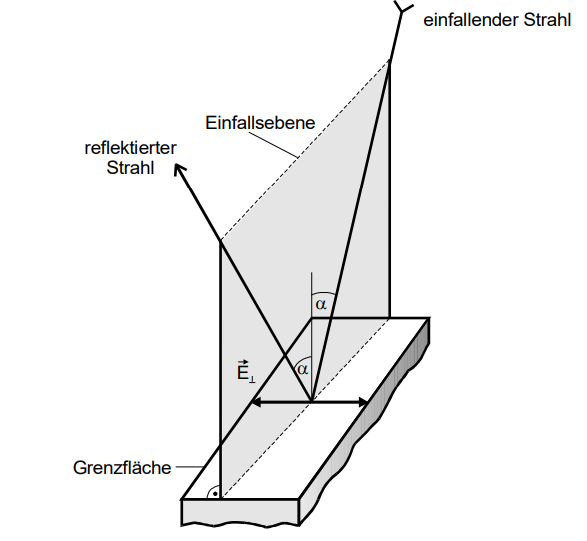
\includegraphics[scale=1]{content/Einfallsebene.png}
    \caption{Perspektivischer Darstellung des Einfalls einer Welle auf eine Grenzfläche \cite{sample}.}
    \label{fig:Einfall}
\end{figure}
\noindent Als letztes muss noch das Verhalten der Komponente $\vec{E}_\parallel$, die in der Einfallsebene schwingt.
In Abbildung \ref{fig:RefanG} ist der Einfall einer in der Einfallsebene polarisierten Lichtwelle eingezeichnet.
Dabei fällt auf, dass auch diese Komponente im Allgemeinen einen tangentialen Anteil besitzt, der sich aus dem Kosinus
des Einfallswinkels ergibt. Dadurch lässt sich auch hier eine Stetigkeitsbedingung
\begin{equation}
    \left(\vec{E}_{\text{e}\parallel}- \vec{E}_{\text{r}\parallel}\right)\cos{\alpha}= \vec{E}_{\text{d}\parallel}\cos{\beta}
    \label{Stetpara}
\end{equation}
aufstellen. Äquivalent zum senkrecht polarisierten Anteil kann nun eine Formel für
den parallel Polarisierten Anteil hergeleitet werden, der nur vom Reflexionswinkel und dem Brechungsindex abhängt.
Die Formel lautet
\begin{equation}
    \vec{E}_{\text{r}\parallel}(\alpha)=\vec{E}_{\text{e}\parallel}\frac{n^2\cos{\alpha}-\sqrt{n^2-\sin^2{\alpha}}}{n^2\cos{\alpha}+\sqrt{n^2-sin^2{\alpha}}}.
    \label{eq:Epara}
\end{equation}
Es lässt sich nun feststellen, dass es einen Winkel $\alpha_\text{p}$ gibt, den sogenannten Brewsterschen Winkel, bei dem kein parallel polarisiertes Licht
reflektiert wird. Also es gilt $\vec{E}_{\text{r}\parallel}(\alpha_\text{p})=0$. Aus dem Brechungsgesetz \eqref{eq:Snellius} lässt sich für den Brewsterschen Winkel folgern, dass
\begin{equation}
    \tan{\alpha_\text{p}}=n
    \label{eq:Brewster}
\end{equation}
gelten muss.\cite{sample}
\begin{figure}[H]
    \centering
    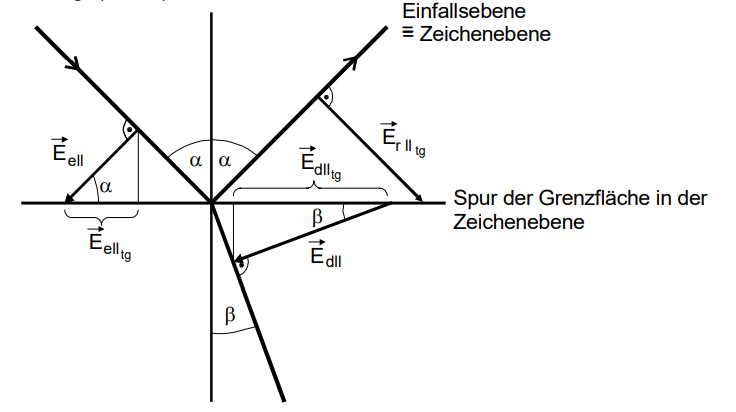
\includegraphics[scale=1]{content/Reflexion.png}
    \caption{Reflexion eines Lichtstrahls, bei dem das E-Feld in der Einfallsebene schwingt \cite{sample}.}
    \label{fig:RefanG}
\end{figure}


